\documentclass{ds-report}
\usepackage{tikz}
\usetikzlibrary{shapes.geometric, arrows, positioning}


\assignment{Distributed Cloud Applications} % Set to `Remote communication` or `Project`.
\authorOne{Jorge Pais} % Name of first team partner.
\studentnumberOne{r0978562} % Student number of first team partner.
\authorTwo{Tomás Maia} % Name of second team partner.
\studentnumberTwo{r0974960}  % Student number of second team partner.

\begin{document}
	\maketitle

    % 1. Imagine you were to deploy your application to a real cloud environment, so not a lab deployment where everything runs on the same machine. Which hosts/systems would then execute which processes, i.e., how are the remote objects distributed over hosts? Clearly outline which parts belong to the front and back end, and annotate with relevant services. Create a component/deployment diagram to illustrate this: highlight where the client(s) and server(s) are.
	\paragraph{Question 1}

Firstly, it is clear that the only front-end component of the application is the web client application, on which users interact indirectly with the API. The client-facing web application which implements a graphical user interface around the API and also has an important role in the authentication process. 

Then the back-end can be split into the following components, which in a real cloud environment would be running in the cloud:

\begin{itemize}
    \item {\bf Booking Platform API:} It is essentially an HTTP API serving as the user/developer facing end of the booking platform's business logic, which is responsible for accessing the back-end services and leveraging the data communication between some of the different components and the API user.
    \item {\bf Firestore Database:} Which is utilised for data persistence, storing not only information about the bookings but also the booked trains, tickets and seats.
    \item {\bf Cloud Pub/sub:} Handles asynchronous indirect messaging between the business logic, specifically on the \texttt{confirmQuote()} method.
    \item {\bf Web Worker Instances:} These are instances of our application which are running in parallel, handling the requests sent to them via Pub/Sub messages.
    \item {\bf External Train Company APIs:} External services used by our application to both read all train-related data and also make requests for booking the tickets.
    \item {\bf Firebase Authentication:} This is the service that is responsible for the application's access management, implementing secure and easy-to-use authentication protocols.  
\end{itemize}

A deployment diagram exemplifying this architecture and the communication that is made by the previous components can be seen in figure \ref{fig:deploymentDiagram}.


    % 2. Where in your application were you able to leverage middleware to hide complexity and speed up development?
    \paragraph{Question 2} 
    We were able to leverage middleware in different parts of our application. Firstly, by using a Spring \texttt{WebClient} it was possible to abstract the low-level details of making HTTP requests and handling the consequent responses since the \texttt{WebClient} can automatically convert the JSON response to an object of a class one can specify.

    Furthermore, \textbf{Cloud Pub/Sub} serves as middleware for enabling indirect communication and decoupling background processes, specifically in our \texttt{confirmQuotes} method. In this way, instead of directly processing confirmation requests, the application makes use of \textbf{Cloud Pub/Sub push subscriptions} and delegates the task to a remote worker.

    We also made use of Cloud Firestore in some of our methods, which acts as middleware for storing and retrieving booking data to a type of NoSQL database. 
    
    Finally, Firebase authentication was utilised in order to implement authentication in a secure way, without having to implement it ourselves, which beside being time consuming could possibly open up our application to security vulnerabilities.

    % 3. At which step of the booking workflow (create quote, collect cart, create booking) would the indirect communication between objects or components kick in? Describe the steps that trigger the indirect communication, and what happens afterwards.
    \paragraph{Question 3}

    During the create quote phase of the booking process, the user selects their travel options and then they receive a quote. This is done by communicating directly with the front-end (the user-facing end) of the API. Next, during the collection of the cart, direct communication is also used, where the user is shown their selections and then they proceed to confirm and create their booking.

    It is at this step where indirect communication is leveraged since the \texttt{confirmQuotes()} method publishes an asynchronous message to the Cloud Pub/Sub service containing all the quotes that are to be booked. This then gets processed by the \texttt{ConfirmQuotesAsync} component of the application, which reads the data and proceeds to book the tickets. Once the booking is successfully created, an acknowledgement message is sent to the Pub/Sub service and the user is notified that their booking was successful.

    % 4. Which kind of data is passed between the application and the background worker when creating a booking? Does it make sense to persist data and only pass references to that data?
    \paragraph{Question 4} 
The message format for PubSub has three attributes: The message data, an ordering key and attributes with additional metadata format. When creating a booking, the data passed between the application and the background worker is a collection of quotes to be confirmed. The quotes are then serialized into JSON format and sent to the publisher inside the data field of the Pub/Sub message. Furthermore, user information, specifically the email address of the user, is also sent as an attribute on the corresponding Pub/Sub message field. This provides context about which user initiated the booking and so that one can then store the bookings in the Cloud Firestore database and associate them with the corresponding user.

Regarding the question of persisting data and passing references, in the current implementation, the actual quote data is serialized and sent. Passing references could be an alternative approach, however, this would require first store the booking details in a database or local storage and then send a reference/identifier to the background workers via Pub/Sub. This could be useful if there happens to be a system crash exactly during the creation of a booking or if the Pub/Sub mechanism fails since the data has already been safely stored. But overall, the extra overhead that is added while writing and reading of the database just to pass references to temporary data might not be worth it in terms of performance and implementation ease.

    % 5. How does your solution to indirect communication improve scalability and responsiveness (especially in a distributed/cloud context)?
    \paragraph{Question 5} 

Using indirect communication in the \texttt{ConfirmQuotes} improves the responsiveness of the service because by using a publish/subscribe model, the system can handle requests asynchronously. The booking process doesn't block the user's session and instead, it proceeds independently in the background, improving the responsiveness of the user interface. 

Also, Cloud Pub/Sub is able to distribute messages across multiple instances of subscriber services, allowing for load balancing to be done. This means that during peak times, more worker instances can be spun up to handle increased message throughput, leading to better scalability.

Besides these advantages, during times of high load, the Pub/Sub system also can absorb a large number of booking requests as messages in the queue. This prevents the back-end services from being overwhelmed.

    % 6. Can you give an example of a user action where indirect communication would not be beneficial in terms of the trade-off between scalability and usability?
    \paragraph{Question 6} 
An example of a user action where indirect communication might not be beneficial due to the trade-off between scalability and usability is the real-time checking of seat availability. In this scenario, where users have a real-time and interactive seat selection interface, where they can see the available seats and their respective states (available, booked, selected), using indirect communication, such as using the Pub/Sub mechanism, could introduce slight delays in delivering real-time updates to the user interface. In scenarios like these, where there is a bigger priority on providing immediate feedback, indirect communication may decrease usability significantly.


    % 7. Is there a scenario in which your implementation of ACID properties may lead to double bookings of one seat?
    \paragraph{Question 7} 

The implementation of the application is geared towards preventing that a user books any ticket of their booking without all tickets in that particular booking being also reserved, thus attempting to guarantee Atomicity. Despite this, there are some cases where the application could get a ticket for a seat and not generate a booking. For example, if a worker instance crashes during the removal process of already "reserved" tickets in a failed booking, this could lead to some of the tickets getting booked, but not removed.

Despite this, a double booking scenario would be unlikely if not impossible, since the moment any of the web workers responsible for creating the booking attempts to do a PUT request on an already booked seat, they won't get a positive HTTP response and as such won't generate a booking.

    % 8. How does role-based access control simplify the requirement that only authorized users can access manager methods?
    \paragraph{Question 8}
Role-based access control allows to define and manage access permissions to certain content based on a user’s role. In this way, it simplifies access management by centralizing and standardizing the granting and revoking of rights.
    
In our particular case, information regarding all the bookings and the best costumers, respectively obtained through the \texttt{getAllBookings} and \texttt{getBestCustomers} methods, are only available for users with the manager role. In this way, instead of granting specific permissions for different users individually, they are simply granted roles whose respective permissions are already pre-established based on certain roles, ensuring security and compliance by guaranteeing that users have access to only the resources and data necessary for their responsibilities. Furthermore, if a user's role changes, the associated permissions of their previous role are instantly revoked.

    % 9. Which components would need to change if you switch to another authentication provider? Where may such a change make it more/less difficult to correctly enforce access control rules, and what would an authentication provider therefore ideally provide?
    \paragraph{Question 9} 

To switch authentication provider from the Firebase one, some changes would have to be made to several components of
the application. First the \texttt{SecurityFilter} class would have to be modified to handle new security tokens/methods, since the current token decode/validate logic is based on JWT tokens.

Also the \texttt{SecurityConfiguration} class would need some modifications in order to integrate the new security provider. The same goes for the \texttt{User} class, which might have to hold a different data structure. The choice of authentication provider may also impact the ease or complexity of implementation. For example, if the new security provider doesn't provide a way to identify a current user's roles within the application, further implementation is also needed in order to get this functionality which was taken for granted with the current Firebase authentication solution.

    % 10. How does your application cope with failures of the Unreliable Train Company? How severely faulty may that train company become before there is a significant impact on the functionality of your application?
    \paragraph{Question 10}
Our application copes with failures of the Unreliable Train Company in different ways. Firstly, when trying to request information about a seat or a train via the \texttt{getSeat} and \texttt{getTrain} methods, respectively, we first check if this information is available in Cloud Firestore. If the seat or train is not found in Cloud Firestore, only then the HTTP request is sent to the Train Company, where we then store the corresponding data in our database, therefore reducing the chances of having a bad response.

Furthermore, to guarantee Atomicity when confirming quotes, i.e. either all quotes are successfully reserved, or none of them are reserved at all, our application has error-handling mechanisms implemented. If a failure occurs when putting tickets, the application attempts to remove the tickets that were previously put. This is done several times until there is a confirmation response that the ticket has been successfully removed.

Regarding the degree of faultiness that the train company may have before there is a significant impact on the functionality of our application, it depends on the specific failure scenarios. For instance, our code attempts to remove tickets up to 25 times in case of a failure, providing a certain level of resilience to temporary faults. However, if the Unreliable Train Company experiences prolonged or consistent return errors, for example consistently failing to put or remove tickets, it might lead to inconsistencies in the state of the application, where customers might have bookings that are not reflected accurately.
    
	\clearpage

\section{Diagrams}

\begin{figure}[h]
    \centering
    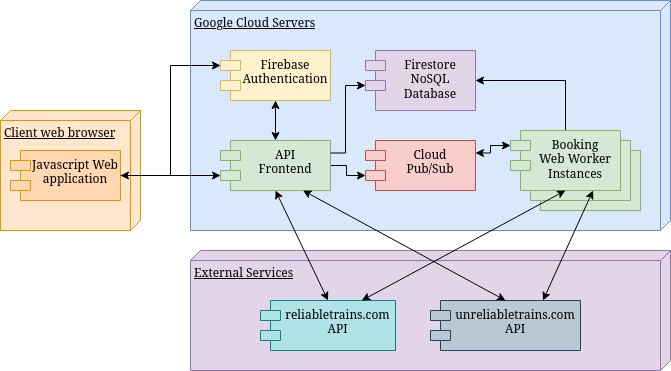
\includegraphics[width = \textwidth]{DeploymentDiagram.png}
    \caption{Deployment Diagram for the developed application}
    \label{fig:deploymentDiagram}
\end{figure}

\begin{thebibliography}{9}

\end{thebibliography}
 
	
\end{document}